\section[Delem]{Het bedrijf Delem}

\index{Delem}Delem werd in 1976 opgericht door de heer H.J.M.M. van Doorne. Op het moment is dit bedrijf de technologische leider op de wereldmarkt in het gebied van besturingen voor metaalbewerkingsmachines. Dit succes komt tot stand door het gebruik van de meest recente techniek in de producten. Delem levert uitsluitend aan OEM\footnote{Original Equipment Manufacturer}-ers (dus de bedrijven die metaalbewerkingsmachines maken) en niet aan eindklanten.

Er zijn ongeveer 60 personen werkzaam bij Delem. Ongeveer 30 hiervan zijn ICT-ers met gemiddeld een WO niveau.

Delem is opgedeeld in een aantal \index{Afdelingen}afdelingen, waarbij de voornaamste development, solutions, \index{Afdelingen!productie}productie en \index{Afdelingen!sales}sales zijn. Uiteraard is er ook nog ondersteunend personeel aanwezig, maar hier wordt verder niet op ingegaan. Een organigram is te vinden op pagina \pageref{organigram}.

In de volgende paragrafen staat een overzicht van de afdelingen die tijdens de stage van belang zijn:

\subsection{Afdeling Development}

\index{Afdelingen!development}Deze afdeling is verantwoordelijk voor het ontwikkelen van nieuwe hard- en software (voor zowel de besturing als voor een PC) en het onderzoeken van nieuwe mogelijkheden voor de besturingen. Gezien de aard van de stage wordt deze dan ook bij deze afdeling uitgevoerd. Zoals tijdens de planning op bladzijde \pageref{planning} te zien is, is er ook tijd gereserveerd voor assistentie voor de andere activiteiten van deze afdeling.

\begin{landscape}
\subsection{Organigram}
\index{Organigram}
\label{organigram}

\begin{figure}[h]{}
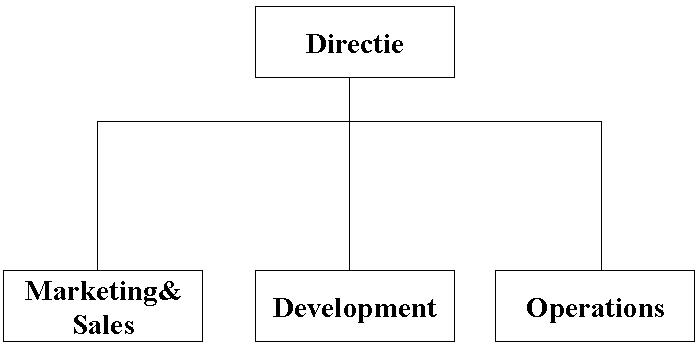
\includegraphics[width=18cm,height=9cm]{organisatie.jpg}
\end{figure}

\end{landscape}

\newpage
